% ============================================================================
% Downhill-Simplex-Algorithmus
% ============================================================================

\ifdefined\outputformat\else\def\outputformat{}\fi
\documentclass[\outputformat]{beamer}

\usetheme[
  pageofpages=von, % String used between the current and the total page count.
  alternativetitlepage=false, % Use the fancy title page.
  titlepagelogo=logo, % Logo for the first page.
]{Torino}

\usepackage[utf8x]{inputenc} % Schriftkodierung mit Umlauten
\usepackage[T1]{fontenc}
\usepackage[ngerman]{babel}
\usepackage{graphicx} % Grafiken
\usepackage{tabularx}
\usepackage{booktabs}
\usepackage{textcomp}
\usepackage{amsmath}
\usepackage{pifont}

\usepackage{multirow} 

\usepackage{bm}
\usepackage{bbm}
\usepackage{color}
\usepackage{tikz}
\usetikzlibrary{arrows,shapes,snakes}

\usepackage{colortbl}

\graphicspath{{abbildungen/}}

%\beamersetuncovermixins{\opaqueness<1>{25}}{\opaqueness<2->{15}}
\logo{
\includegraphics[height=0.0625\paperheight]{HSR_Logo_CMYK.pdf}}

\author{Selina Malacarne \and\\ Raphael Nestler}
\title{Simplex Algorithmus für nichtlineare Optimierungsprobleme}
\subtitle{Simplex-Downhill Algorithmus}
%\institute{
\includegraphics[height=0.13\paperheight]{HSR_Logo_CMYK.pdf}}
\date{13. Mai 2013}

\setcounter{tocdepth}{1}

% ============================================================================
\begin{document}

\begin{frame}
\titlepage
\end{frame}

\begin{frame}{Programm}
\tableofcontents
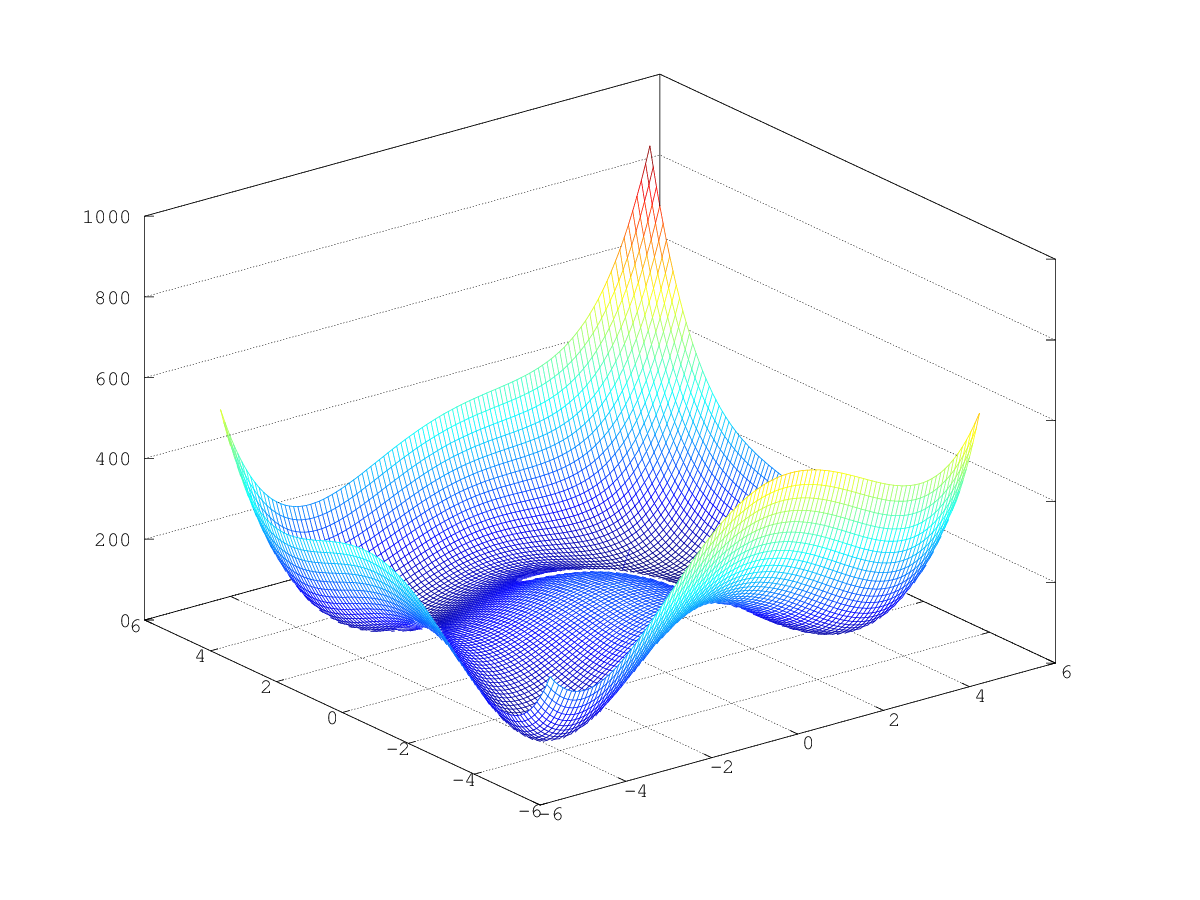
\includegraphics[height=0.5\paperheight]{himmelblau.png}
\end{frame}

% ============================================================================
\section{Einleitung} 
\begin{frame}{Programm}\tableofcontents[currentsection]\end{frame}

\begin{frame}{Grundlagen}
\begin{itemize}
	\item Beschrieben von John Nelder und Roger Mead ($\approx 1965$)
	\item \textbf{NICHT} verwechseln mit Simplex Algorithmus
	\item Anwendung: 
	\begin{itemize}
		\item Optimierung nichtlinearer Funktionen mit mehreren Parametern 
		\item Kurvenfitten (bspw. Messwerte an Kurve angleichen)
	\end{itemize}	
	\item Kategorie: Hillclimbing- oder Downhill Suchverfahren
\end{itemize}
\end{frame}

\begin{frame}{Merkmale}
\begin{itemize}
	\item Vergleicht mehrere Punkte (N-Dimensionen+1)
	\item Verwendung von \textbf{einfachst möglichen Volumina} (Simplex $\rightarrow$ bei n=2: Simplex = Dreieck)
	\item Vorteile
	\begin{itemize}
		\item Benötigt \textbf{keine} Ableitungen
		\item Einfach und robust
	\end{itemize}
	\item Nachteile
	\begin{itemize}
		\item Langsam (konvergiert linear)
		\item Kann in lokales Minima fallen
	\end{itemize} 
\end{itemize}
\end{frame}

% ============================================================================
\section{Der Algorithmus} 
\begin{frame}{Programm}\tableofcontents[currentsection]\end{frame}

\begin{frame}{Übersicht}
\newcommand{\highlight}{white}

%\usetikzlibrary{arrows}
\begin{tikzpicture}[node distance = 1.7cm,every node/.style={rectangle,fill=white},
  block/.style={draw},
  highlight/.style={draw,fill=\highlight},
  line/.style = {draw,-latex'}
]

\node (start) [block] {N+1 Startpunkte $x_i$ wählen (Simplex bilden)};

\node (a1) [block, below of=start] { $y_i = f(x_i)$ berechnen};

\node (a2) [block, below of=a1] { Bestes ($y_{min}$) und schlechtestes ($y_{max}$) $y_i$ bestimmen};

\node (a3) [block, below of=a2 ]{$y_{min}$ gut genug?};

\node (ende) [block, below of=a3] {Ende};

\node (a4) [highlight, left of=a3, node distance=6cm] {Neuer Simplex bilden};



\path[line] (start) -- (a1);
\path[line] (a1) -> (a2);
\path[line] (a2) -> (a3);

\path[line] (a3) -> node{ja} (ende);
\path[line] (a3) -> node{nein} (a4);

\path[line] (a4)  |-  (a1.west);

\end{tikzpicture}

\end{frame}
\begin{frame}{Übersicht}
\newcommand{\highlight}{green}

%\usetikzlibrary{arrows}
\begin{tikzpicture}[node distance = 1.7cm,every node/.style={rectangle,fill=white},
  block/.style={draw},
  highlight/.style={draw,fill=\highlight},
  line/.style = {draw,-latex'}
]

\node (start) [block] {N+1 Startpunkte $x_i$ wählen (Simplex bilden)};

\node (a1) [block, below of=start] { $y_i = f(x_i)$ berechnen};

\node (a2) [block, below of=a1] { Bestes ($y_{min}$) und schlechtestes ($y_{max}$) $y_i$ bestimmen};

\node (a3) [block, below of=a2 ]{$y_{min}$ gut genug?};

\node (ende) [block, below of=a3] {Ende};

\node (a4) [highlight, left of=a3, node distance=6cm] {Neuer Simplex bilden};



\path[line] (start) -- (a1);
\path[line] (a1) -> (a2);
\path[line] (a2) -> (a3);

\path[line] (a3) -> node{ja} (ende);
\path[line] (a3) -> node{nein} (a4);

\path[line] (a4)  |-  (a1.west);

\end{tikzpicture}

\end{frame}



% ============================================================================
\section{Strom/Spannung-Kennlinie aufnehmen}
\begin{frame}{Programm}\tableofcontents[currentsection]\end{frame}

\begin{frame}{Messen von U/I-Kennlinien (S.15)}

\end{frame}


\end{document}
